\documentclass[runningheads]{llncs}
\usepackage[T1]{fontenc}
\usepackage{amsmath}
\usepackage{amssymb}
\usepackage{xcolor}
\usepackage{tikz}
\usetikzlibrary{math, automata, positioning}

\begin{document}

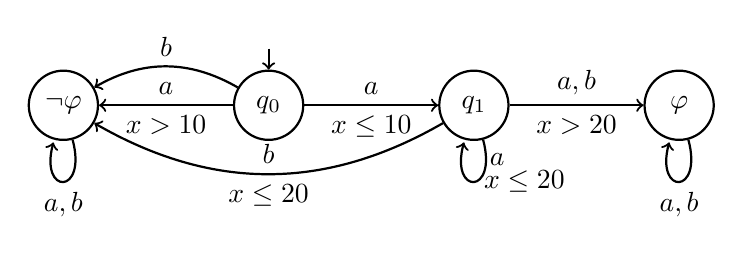
\begin{tikzpicture} [node distance = 1.7cm, thick]
    \node (q0)     [state, initial text={}]          {$q_0$};
    \node (i)   at (0,.85) {};
    \node (q1)     [state, right = of q0]    {$q_1$};
    \node (phi)    [state, right = of q1]    {$\varphi$};
    \node (notphi) [state, left = of q0]    {$\neg\varphi$};
    
    \draw[->, thick] (i) edge (q0);
     \draw[->, thick] (q0) edge node[above] {$a$} node[below]{$x \leq 10$} (q1);
     \draw[->, thick] (q1) edge node[above] {$a, b$} node[below]{$x > 20$} (phi);

     \draw[->, thick] (q0) edge[bend right=30] node[above]{$b$} (notphi);
     \draw[->, thick] (q0) edge[] node[above]{$a$} node[below]{$x > 10$} (notphi);

     \draw[->, thick] (q1) edge[bend left=30] node[above]{$b$}  node[below]{$x\leq20$} (notphi);
    
    \draw[->, thick] (phi) edge [loop below] node[] {$a,b$} (phi);
    \draw[->, thick] (q1) edge [loop below] node[above right=0.1cm] {$a$} node[right] {$x \leq 20$} (q1);
    \draw[->, thick] (notphi) edge[loop below] node[]{$a,b$} (notphi);

\end{tikzpicture}

\end{document}